\documentclass{article}

\usepackage{shared}

\usepackage{biblatex}
\addbibresource{references.bib}

\title{SCARV: RISC-V Crypto ISE \\ Reference Implementation}

\begin{document}

%% Custom Commands %%

% For multi-line autoflowed table cells
\newcolumntype{Y}{>{\RaggedRight\arraybackslash}X}

% Table of interface signals.
\newcommand{\SIGNALS}[3]{
\begin{table}[H]
\begin{tabularx}{\textwidth}{@{} c c l Y @{}}
\toprule
\textbf{I/O} & \textbf{Size} & \textbf{Name} & \textbf{Description} \\
\midrule
#1
\bottomrule
\end{tabularx}
\caption{#2}
\label{#3}
\end{table}
}

% Reference to a signal name
\newcommand{\SIGREF}[1]{{\tt #1}}

% Input interface signal
\newcommand{\SIGNALI}[3]{
    {\bf I} & $#1$ &{\tt #2}& #3 \\ \addlinespace
}

% Output interface signal
\newcommand{\SIGNALO}[3]{
    {\bf O} & $#1$ &{\tt #2}& #3 \\ \addlinespace
}

% Common section / name references
\newcommand{\cpucopif}{\nameref{sec:cpu-cop-if} }

%% End Custom Commands %%

\maketitle

\abstract{
This document contains the micro-architectural specification for an
implementation of the RISC-V Crypto ISE.
}
\tableofcontents

\section{Introduction}

This document contains the design specification for an {\em area optimised}
implementation of the proposed RISC-V Crypto ISE (C-ISE).

The implementation takes the form of a Co-processor (COP), which is designed
to make it extremely easy to re-use, and integrate with existing RISC-V cores
which support custom ISEs. We define the interfaces to the Co-processor, as
well as it's internal micro-architecture and how to integrate it with an
existing CPU core.

Note that this is only a reference implementation. It is not the only way
to implement the ISE, nor is it the best for any given set of design
constraints. It would be perfectly acceptable to create a single CPU core
which tightly integrates the ISE into it's execution pipeline (as one might
with a core supporting the floating-point F extension), rather than
attatching to it as a co-processor. There are numerous performance and
efficiency improvements to be had from such an approach. We used a
co-processor architecture because it make re-use with existing CPU designs
(such as picorv32 or Rocket) much easier.

The rest of the document is structured as follows: Section 
\ref{sec:cop-interfaces} describes the interfaces of the COP. Section
\ref{sec:cop-microarch} describes the internal organisation of the COP.
Section \ref{sec:integration} details how to integrate the COP into an
existing RISC-V processor design. Section \ref{sec:verification} describes
how the COP implementation was verified.

\section{COP Interfaces}
\label{sec:cop-interfaces}

Here, we detail the interfaces to the COP. By defining this interface, we
hope that others can modify the internals of the COP to suite their own
design constraints, and still have a drop-in compatible design.

\subsection{Clock and Reset Interface}
\label{sec:if-clk-reset}

\SIGNALS{
\SIGNALI{1}{g\_clk}{The global input clock signal.}
\SIGNALO{1}{g\_clk\_req}{
COP clock request signal. The COP sets this signal high when it needs a
clock signal, and clears it when it does not. Used to indicate the COP
is idle.
}
\SIGNALI{1}{g\_resetn}{Synchronous, active low reset signal.}
}{}{tab:sigs-clk-reset}

\subsection{Status Interface}

TBD

\subsection{CPU/COP Interface}
\label{sec:cpu-cop-if}

The CPU/COP interface is the channel through which the CPU can send
instructions to the COP and recieve results.
The four signals
{\tt cpu\_insn\_req, cop\_insn\_ack, cpu\_insn\_ack} and
{\tt cop\_insn\_rsp}
control the rate of information flow between the CPU and the COP.

\subsubsection{Signal List}

\SIGNALS{
\SIGNALI{1}{cpu\_insn\_req}{
    Set by the CPU to indicate a new instruction needs to be executed.
    There must be no combinatorial path from {\tt cpu\_insn\_req} to  
    {\tt cop\_insn\_ack}.
}
\SIGNALO{1}{cop\_insn\_ack}{
    Co-processor acknowledge. This is asserted by the co-processor to say
    that it has received the data from the CPU and will start working on the
    supplied instruction.
}
\SIGNALI{1}{cpu\_abort\_req}{
    Set by the CPU to tell the COP to abort whatever instruction it is
    executing (if any) and return to an idle state where it is ready to
    accept new instructions. This signal is used to abort long multi-cycle
    instructions in the presence of a pending interrupt.
    There must be no combinatorial path from {\tt cpu\_insn\_abort} to
    {\tt cop\_insn\_ack}.
}
\SIGNALI{32}{cpu\_insn\_enc}{
    The encoded instruction word to be executed by the COP.
}
\SIGNALI{32}{cpu\_rs1}{
    The value of $\GPR$ source 1 ({\tt rs1}), which is used as the source
    register for some ISE instructions. The CPU only needs to provide this
    for a very small subset of the ISE instructions: \ASM{SB.cr, SH.cr,
        SW.cr, SCATTER.x, GATHER.x} and \ASM{MV2CPR}.
}
\SIGNALO{1}{cop\_wen}{
    Co-processor write enable, indicates to the CPU that a value needs to
    be written from the co-processor {\tt cop\_wdata} signal into the
    RISC-V GPR register addressed by {\tt cop\_waddr}.
}
\SIGNALO{5}{cop\_waddr}{
    The RISC-V GPR destination register address used by the COP instructions
    \ASM{MV2GPR, EQU.mp, LTU.MP} and \ASM{GTU.mp}.
}
\SIGNALO{32}{cop\_wdata}{
    The data to be written to the RISC-V GPR register addressed by 
    {\tt cop\_waddr} by the 
    \ASM{MV2GPR, EQU.mp, LTU.MP} and \ASM{GTU.mp}
    instructions.
}
\SIGNALO{3}{cop\_result}{
    This signal encodes the result of the executed instruction: whether
    it succeeded or, if it raised an exception, what kind. The encodings
    are described in table \ref{tab:cop-result-encodings}.
}
\SIGNALO{1}{cop\_insn\_rsp}{
    Co-processor response. Used to indicate processing of the current
    instruction has finished and that we are ready for the next one. Writeback
    and response data is valid when this signal is set.
    There must be no combinatorial path from {\tt cpu\_insn\_rsp} to
    {\tt cpu\_insn\_ack}.
}
\SIGNALO{1}{cpu\_insn\_ack}{
    Allows the CPU to signal to the co-processor it has recieved all
    information from the execution of an instruction.
}
}{}{tab:sigs-cpu-cop}


\begin{table}[h!]
\centering
\begin{tabular}{ll}
\toprule
{\bf Result Code} & {\bf Meaning} \\
\midrule
 {\tt 0b000}  & Success \\
 {\tt 0b001}  & Aborted \\
 {\tt 0b010}  & Instruction decode exception \\
 {\tt 0b100}  & Load address misaligned exception  \\
 {\tt 0b101}  & Store address misaligned exception \\
 {\tt 0b110}  & Load access fault                  \\
 {\tt 0b111}  & Store access fault                 \\
 \bottomrule
\end{tabular}
\caption{Encodings for the \SIGREF{cop\_result} signal. All other encoding
values are reserved and should not be used.}
\label{tab:cop-result-encodings}
\end{table}

\subsubsection{Example Transactions}

This section gives a non-exhaustive list of timing diagrams for example
transactions over the CPU/COP interface.

\begin{figure}[H]
\centering
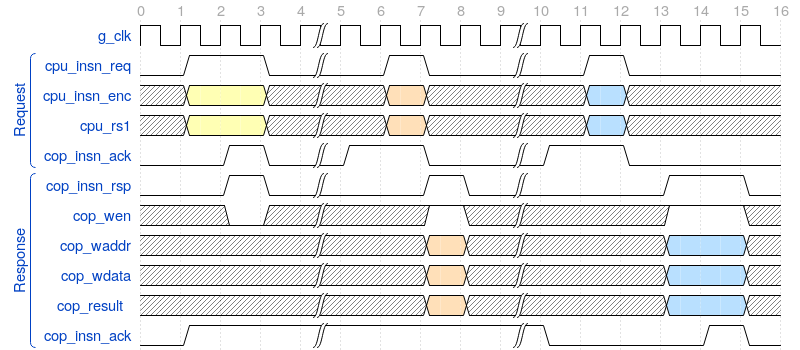
\includegraphics[width=\textwidth]{./diagrams/cpu-cop-if-1.png}
\caption{Simple instruction request, acknowledge, result with delays.
The first transaction shows an instruction request in cycle 1, followed
by the acknlowedgement and result in cycle 2.
The second shows that if {\tt cop\_insn\_ack} is set already, then
instructions can be accepted immediately and their result returned on the next
cycle.  The third shows how the request / acknowledge protocol handles
stalls.}
\label{fig:cpu-cop-if-waves-1}
\end{figure}

\begin{figure}[H]
\centering
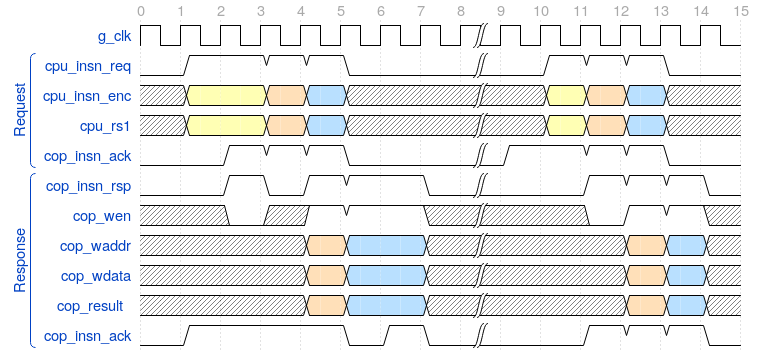
\includegraphics[width=\textwidth]{./diagrams/cpu-cop-if-2.png}
\caption{This figure shows the same three transactions as in figure
\ref{fig:cpu-cop-if-waves-1} but with the requests issued back to back.
In the set of transactions, the results of each transacton are not always
accepted on the next cycle. In the second set, we see the interface working
at maximum throughput, with every request accepted in the same cycle, and
results always accepted in the next cycle.}
\end{figure}



\subsection{Memory Interface}
\label{sec:mem-if}

The COP uses a single extra memory interface in order to implement the
load/store instructions. It is a simple SRAM-style interface which can be
connected directly to a BRAM, converted into a bus interconnect (AXI4-Lite
for example) or multiplexed with the CPU data memory interface.

The interface uses a 32-bit, word aligned address. Misaligned accesses
are {\em not} supported in this implementation of the ISE and will raise
a {\em misaligned load/store exception} via the CPU/COP interface.

\subsubsection{Signal List}

These signals are synchronous with the {\tt g\_clk} signal described in
section \ref{sec:if-clk-reset}.

\SIGNALS{
\SIGNALO{1}{cop\_mem\_cen}{
    Memory chip enable, signaling an active transaction. When asserted this
    signal must stay set until the following cycle, where it can be cleared
    iff {\tt cop\_mem\_stall} is clear. If the stall signal is not clear, it
    must remain set until either stall is clear, or {\tt cop\_mem\_error}
    is high.
}
\SIGNALO{1}{cop\_mem\_wen}{
    Memory write enable. Must remain stable during a transaction.
}
\SIGNALO{32}{cop\_mem\_addr}{
    Memory address. Must remain stable during a transaction.
}
\SIGNALO{32}{cop\_mem\_wdata}{
    Memory write data. Must remain stable during a transaction.
}
\SIGNALO{4}{cop\_mem\_ben}{
    Memory byte enable. On a write, this indicates which bytes in the word
    are to be updated. On a read, this indicates which bytes of the word we
    are looking to have returned. Must remain stable during a transaction.
}
\SIGNALI{32}{cop\_mem\_rdata}{
    Memory read data.
}
\SIGNALI{1}{cop\_mem\_stall}{
    Memory stall, indicating the COP must wait another cycle for the response.
}
\SIGNALI{1}{cop\_mem\_error}{
    Memory error. Indicates the COP has tried to access unmapped or otherwise
    invalid memory space. The error signal can only be asserted when the
    chip enable is high in the previous cycle. The chip enable must be
    cleared when the error signal is asserted.
}
}{}{tab:sigs-mem}

\subsubsection{Example Transactions}

\begin{figure}[H]
\centering
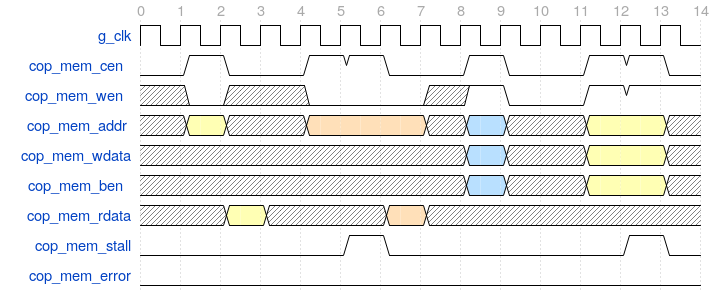
\includegraphics[width=\textwidth]{./diagrams/cop-mem-if-1.png}
\caption{This timing diagram shows a read, followed by a stalled read,
followed by a write, and finally a stalled write on the COP memory interface.
Note that {\tt cop\_mem\_cen} remains high for only a single cycle in a
non-stalled transaction, but must remain high while the stall signal is also
asserted.}
\label{fig:cop-mem-if-waves-1}
\end{figure}

\begin{figure}[h]
\centering
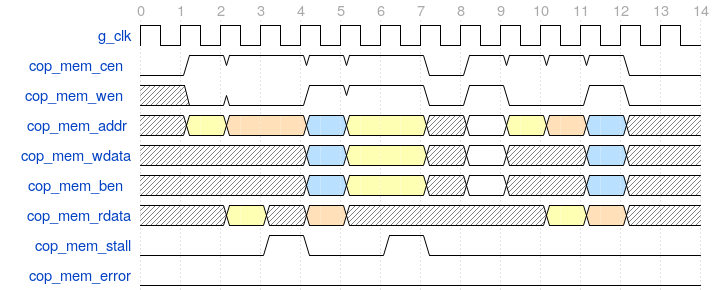
\includegraphics[width=\textwidth]{./diagrams/cop-mem-if-2.png}
\caption{This timing diagram shows the same set of transactions as in
\ref{fig:cop-mem-if-waves-1} but back-to-back with no intervening cycles
where the bus is idle.}
\label{fig:cop-mem-if-waves-2}
\end{figure}


\section{COP Internal Micro-architecture}
\label{sec:cop-microarch}

This section describes the main internal blocks and interfaces of the COP.

\begin{figure}[H]
\centering
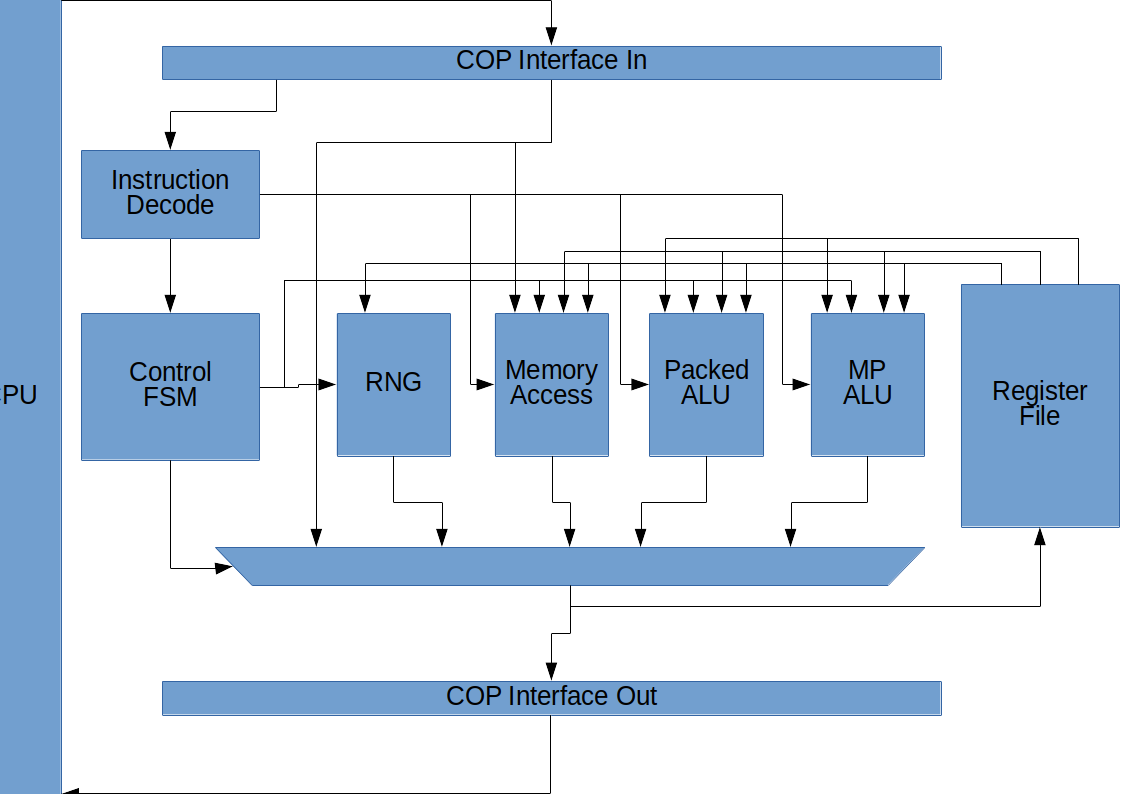
\includegraphics[width=0.7\textwidth]{diagrams/cop-block-diagram.png}
\caption{A block diagram of the main components and data paths of
the COP.}
\label{fig:cop-block-diageam}
\end{figure}

\subsection{Instruction Decode Block}

This block is responsible for taking the 32-bit encoded instructions from
the \cpucopif and extracting the relevent fields for each instruction. This
will be a highly re-usable block.

This block will be completely combinatorial. It will be up to the wider
environment to register it's inputs and outputs as needed. Not all of the
decoded output fields will be valid for every instruction.

\SIGNALS{
\SIGNALI{32}{id\_encoded}{
    The encoded 32-bit instruction word. This signal should be kept as stable
    as possible, as any toggling will affect a large amount of down-stream
    logic.
}
\SIGNALO{ 1}{id\_exception}{
    This signal is asserted iff the presented \SIGREF{id\_encoded} signal
    does not represent a valid ISE instruction.
}
\SIGNALO{ 3}{id\_class}{
    Indicates which class the decoded instruction belongs too. This is used
    to very quickly indicate which functional unit will be needed to execute
    the instruction. Encodings for this signal are found in table
    \ref{tab:id-class-encodings}.
}
\SIGNALO{ 4}{id\_subclass}{
    Identifies the individual instruction within a particular class (as
    described by \SIGREF{id\_class}) so it can be executed.
}
\SIGNALO{ 3}{id\_pw}{
    Decoded pack width for packed arithmetic instructions.
}
\SIGNALO{ 4}{id\_crs1}{Decoded crypto ISE source register 1.}
\SIGNALO{ 4}{id\_crs2}{Decoded crypto ISE source register 2.}
\SIGNALO{ 4}{id\_crs3}{Decoded crypto ISE source register 3.}
\SIGNALO{ 4}{id\_crd1}{Decoded crypto ISE desgination register 1.}
\SIGNALO{ 4}{id\_crd2}{
    Decoded crypto ISE desgination register 2. Only used by the
    multi-precision instructions.
}
\SIGNALO{ 5}{id\_rd}{
    Destination register for instructions which write to the RISC-V
    GPRs.
}
\SIGNALO{ 5}{id\_rs1}{
    Source register for instructions which source from the RISC-V
    GPRs.
}
\SIGNALO{32}{id\_imm}{
    The decoded immediate value for the instruction. This value encodes
    all the kinds of immediate which are packed into the encoded instruction.
    \begin{itemize}
    \item Load/Store Offsets.
    \item Shift amounts for packed and multi-precision instructions.
    \item LUT values for {\tt BOP.cr}
    \item Positions and sizes for bitfield instructions {\tt INS.cr}
          and {\tt EXT.cr}.
    \item {\tt LLI.cr} and {\tt LUI.cr} Immediates.
    \item Twiddle positions.
    \end{itemize}

    For load and store offsets, the encoded immediates are also
    sign-extended.
}
}{
    Input and output signals to the crypto ISE instruction decode block.
}{tab:sigs-decode-block}

\begin{table}[h!]
\centering
\begin{tabular}{ll}
\toprule
{\bf \SIGREF{id\_class} code} & {\bf Instruction Class} \\
\midrule
 {\tt 0b???}  & Packed Arithmetic \\
 {\tt 0b???}  & Twiddle           \\
 {\tt 0b???}  & Load / Store      \\
 {\tt 0b???}  & Random            \\
 {\tt 0b???}  & Move              \\
 {\tt 0b???}  & Multi-precision   \\
 {\tt 0b???}  & Bitwise           \\
 \bottomrule
\end{tabular}
\caption{Encodings for the \SIGREF{id\_class} signal. All other encoding
values are reserved and should not be used.}
\label{tab:id-class-encodings}
\end{table}

There is considerable scope in this block for optimisation in terms of
energy efficiency. Gating the input wires to different parts of the decode
tree and output signals depending on the decoded instruction will have a
large impact on power expended decoding sequences of instructions.

\subsection{COP Register File}

We use a four port register file.
Three ports are 32-bit dedicated read-ports.
One port is a 32-bit dedicated write port.
The register file has extra signals which allow individual bytes and
halfwords of each register word to be written in isolation.

\SIGNALS{
\SIGNALI{ 1}{crs\_[1|2|3]\_ren  }{Register read port enable}
\SIGNALI{ 4}{crs\_[1|2|3]\_addr }{Register read port address}
\SIGNALO{32}{crs\_[1|2|3]\_rdata}{Register read data}
}{
Interface signals for the register file read ports.
All signals are synchronous to \SIGREF{g\_clk}.
}{tab:sigs-regfile-read}

\SIGNALS{
\SIGNALI{ 4}{crd\_wen  }{Register byte write port enable}
\SIGNALI{ 4}{crd\_addr }{Register write port address}
\SIGNALO{32}{crd\_wdata}{Register write data}
}{
Interface signals for the register file write port.
All signals are synchronous to \SIGREF{g\_clk}.
The 4-bit \SIGREF{crd\_wen} signal is a per-byte lane write enable
signal. Byte $i$ of \SIGREF{creg\_d\_wdata} is only written back if
bit $i$ of the write enable signal is set.
}{tab:sigs-regfile-write}

Though many of the COP instructions are implemented using micro-code
they can still be issued to the COP back to back.
This means the implementation must still handle {\em RAW} hazards
with forwarding logic, or stall for a cycle to allow all writebacks
to occur.

\subsection{Packed Arithmetic Block}

This block is responsible for implementing all of the packed arithmetic,
twiddle, conditional move and bitwise instructions.

It takes upto three 32-bit input words from the register file, and the sign
extended immediate (if any) from the instruction decode block.
It produces a single 32-bit result corresponding to the operation it
performed.

\SIGNALS{
\SIGNALI{1}{palu\_ivalid}{
    Indicates that the input instruction data is valid and that the 
    block should execute the specified instruction.
}
\SIGNALO{1}{palu\_idone}{
    Indicates that the block has finished executing an instruction
    and is ready for another on the next cycle.
}
\SIGNALI{32}{palu\_rs1}{Register operand 1}
\SIGNALI{32}{palu\_rs2}{Register operand 2}
\SIGNALI{32}{palu\_rs3}{Register operand 3}
\SIGNALI{32}{id\_imm}{
    Decoded instruction immediate. Includes the 16-bit operands for
    {\tt LLI/LUI}, shift distances and the 4-bit LUT for {\tt BOP}.
}
\SIGNALI{4}{id\_class}{
    Identifies which class of instruction the COP is executing.
}
\SIGNALI{3}{id\_subclass}{
    Identifies which instruction is being executed by the packed ALU block.
}
\SIGNALO{4}{palu\_cpr\_rd\_ben}{
    4-bit byte write enable signal for writeback data.
}
\SIGNALO{32}{palu\_cpr\_wdata}{
    Data to be written to the $\CPR$ register file
}
\SIGNALO{32}{palu\_cpr\_wen}{
    Packed ALU $\CPR$ write enable.
}
}{Interface signals for the packed arithmetic block. All signals are
synchronous to \SIGREF{g\_clk}.}
{tab:sigs-pack-arith-block}

The operation performed is specified by the control FSM.
This includes the pack width being operated on, and the LUT used for bitwise
operations.

\subsection{Multi-precision Arithmetic Block}

This block is responsible for implementing all of the multi-precision
arithmetic and comparison instructions.

The block can source upto two registers at a time.
It can write a single 32-bit value at a time.
This puts a lower bound on the latency of most multi-precision instructions.
The latency is acceptable in an area-optimised implementation and still
makes the block more performant than the equivalent RISC-V instruction
sequence.

\SIGNALS{
\SIGNALI{1}{malu\_ivalid}{
    Indicates that the input instruction data is valid and that the MP ALU 
    block should execute the specified instruction.
}
\SIGNALO{1}{malu\_idone}{
    Indicates that the MP ALU has finished executing an instruction
    and is ready for another on the next cycle.
}
\SIGNALI{32}{cpr\_rs1}{Register operand 1}
\SIGNALI{32}{cpr\_rs2}{Register operand 2}
\SIGNALI{32}{cpr\_rs3}{Register operand 3}
\SIGNALI{4}{id\_class}{
    Identifies which class of instruction the COP is executing.
    The MP ALU block only looks for the Multi-precision
    class as per table \ref{tab:id-class-encodings}.
    All others are ignored.
}
\SIGNALI{3}{id\_subclass}{
    Identifies which instruction is being executed by the memory block.
}
\SIGNALI{32}{id\_imm}{
    Decoded instruction immediates. Used by the MP ALU block for immediate
    shift amounts.
}
\SIGNALO{4}{malu\_cpr\_rd\_ben}{
    4-bit byte write enable signal for writeback data.
}
\SIGNALO{32}{malu\_cpr\_wdata}{
    Data to be written to the $\CPR$ register file
    Results from the MP ALU are written back over two cycles.
    The low-word of a result is always written back first.
    The destination register is controlled by the FSM block.
    It is possible to overlap writing back of the low word with computing
    the high word value in some cases.
}
\SIGNALO{32}{malu\_cpr\_wen}{
    MP ALU block $\CPR$ write enable. There may be multiple writes to
    the $\CPR$ register file per instruction.
}
}{Interface signals for the multi-precision arithmetic block. All signals are
synchronous to \SIGREF{g\_clk}.}
{tab:sigs-multi-arith-block}

The block contains a single 64-bit {\tt scratch} register.
This is used to store intermediate results during computation.

The table below shows roughly what the ALU does in each cycle during
instruction execution.

\begin{table}[H]
\begin{tabularx}{\textwidth}{l Y Y Y }
\toprule
\textbf{Instruction}& \textbf{Cycle 0}& \textbf{Cycle 1}& \textbf{Cycle 2} \\
\midrule
ADD2.mp&
    $scratch \ASN rs1+rs2;$\newline 
    $rdm0\ASN scratch[31:0]$ 
 &  $rdm1\ASN scratch[32]$ 
 & \\
ADD3.mp&
   $scratch \ASN rs1 + rs2$
 & $scratch \ASN scratch + rs3;$\newline
   $rdm0\ASN scratch[31:0]$ 
 & $rdm1\ASN scratch[63:32]$ 
\\
SUB2.mp&
 &
 &
\\
SUB3.mp&
 &
 &
\\
ACC1.mp&
 &
 &
\\
ACC2.mp&
 &
 &
\\
MAC.mp &
 &
 &
\\
MAA.mp &
 &
 &
\\
SLLI.mp&
 &
 &
\\
SLLR.mp&
 &
 &
\\
SRLI.mp&
 &
 &
\\
SRLR.mp&
 &
 &
\\
EQU.mp &
 &
 &
\\
LTU.mp &
 &
 &
\\
GTU.mp &
 &
 &
\\
\bottomrule
\end{tabularx}
\caption{Table showing what the multi-precision ALU does in each cycle
per instruction execution. Here, $rdm0$ refers to the low word of the
destination register pair, and $rdm1$ to the high word.}
\label{tab:mp-alu-exec}
\end{table}

\subsection{Memory Block}

The memory block is responsible for all instruction which access main
memory.

It contains it's own FSM for controlling the memory interface
and particularly the {\tt SCATTER.x} and {\tt GATHER.x} instructions.
The states and transitions for the FSM are shown in figure 
\ref{fig:mem-block-fsm}. 
In the figure, edges labled {\em launch} are
where memory transactions are started.
{\em Stall} edges are used to
account for cycles where the memory interface does not respond immediately.
{\em Finish} edges are when we assert that an instruction has finished
execution.

In order to launch a new transaction, both the \SIGREF{cop\_mem\_stall}
and \SIGREF{cop\_mem\_error} signals must be clear on the
\nameref{sec:mem-if}.

\begin{figure}
\centering
\includegraphics[width=1.0\textwidth]{diagrams/fsm-load-store.eps}
\caption{State transition diagram for the memory interface block.
Note that memory transactions will always be launched when exiting the
{\tt IDLE} state. There is also an implicit edge from every state to
{\tt IDLE} indicating an error and subsequent transaction abort.}
\label{fig:mem-block-fsm}
\end{figure}

The memory block is responsible for driving the \nameref{sec:mem-if}.
In addition to those siganls, the block also has the following signals
listed in table \ref{tab:sigs-mem-block}.

\SIGNALS{
\SIGNALI{1}{mem\_ivalid}{
    Indicates that the input instruction data is valid and that the memory
    block should execute the specified instruction.
}
\SIGNALO{1}{mem\_idone}{
    Indicates that the Memory Block has finished executing an instruction
    and is ready for another on the next cycle.
}
\SIGNALO{1}{mem\_addr\_error}{
    When set, indicates an address misalignment error on the bus.
    Valid only when \SIGREF{mem\_idone} is set.
}
\SIGNALO{1}{mem\_bus\_error}{
    When set, indicates a bus error / memory fault exception.
    Valid only when \SIGREF{mem\_idone} is set.
}
\SIGNALI{4}{id\_class}{
    Identifies which class of instruction the COP is executing.
    The Memory block only looks for the Load/Store and Scatter/Gather
    classes as per table \ref{tab:id-class-encodings}.
    All others are ignored.
}
\SIGNALI{3}{id\_subclass}{
    Identifies which instruction is being executed by the memory block.
}
\SIGNALI{32}{id\_imm}{
    The decoded offset immediate. Used for load/store offsets.
}
\SIGNALI{32}{gpr\_rs1}{
    Source register 1 from the RISC-V GPR file. Used as the base address
    for all memory accesses.
}
\SIGNALI{32}{cpr\_rs1}{
    Crypto source register 1.
}
\SIGNALI{32}{cpr\_rs2}{
    Crypto source register 2.
}
\SIGNALO{4}{mem\_cpr\_rd\_ben}{
    4-bit byte write enable signal for writeback data.
}
\SIGNALO{32}{mem\_cpr\_wdata}{
    Data to be written to the $\CPR$ register file
}
\SIGNALO{32}{mem\_cpr\_wen}{
    Memory block $\CPR$ write enable. There may be multiple writes to
    the $\CPR$ register file per instruction.
}
}{
    IO signals for the Memory Block, excluding those from the 
    \nameref{sec:mem-if}. All signals are synchronous to {\tt g\_clk}.
}
{tab:sigs-mem-block}

\subsection{RNG Block}

The RNG block acts as a random number source. It interacts with only the
{\tt RSAMP.cr} and {\tt RSEED.cr} instructions.

{\bf TBD:} {\em Decide what sort of random number source we will use in
the implementation.}

\section{Integration Guide}
\label{sec:integration}

TBD

\section{Verification}
\label{sec:verification}
\import{./}{ise-verification.tex}

\printbibliography


\end{document}
